\section{Black Hole Fundamental Plane in Illustris}

\label{sec:analysis}Starting with our sample of black holes from
the Illustris simulation, we seek a relation between the masses and
accretion rates. This relation allows us to construct a power-law
relationship between $M$ and $\dot{M}$ using linear least-squares
(Figure \ref{fig:bhpop_hist2d}). The best-fit is given by

\begin{equation}
\log\dot{M}=0.869\log M_{BH}-17.855.\label{eq:int_relation}
\end{equation}
This relationship reflects the intrinsic properties of the simulation,
and is independent of any models.
\begin{figure}
\centering{}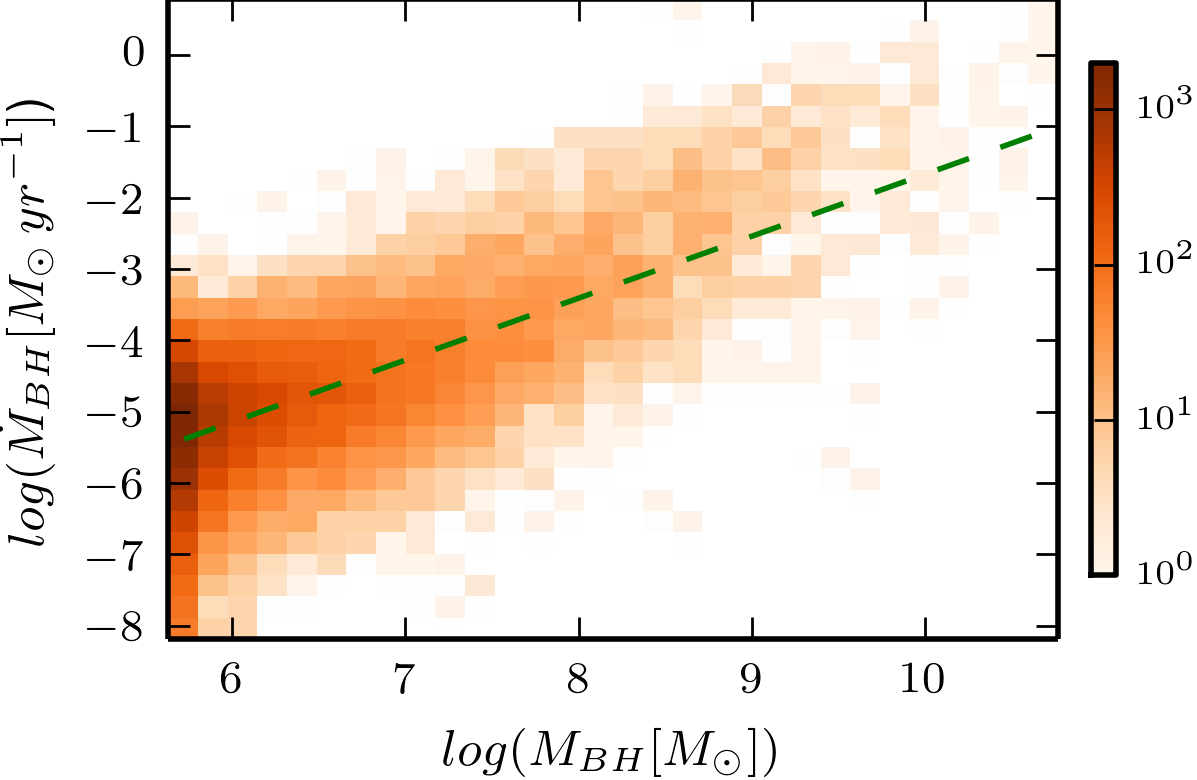
\includegraphics[clip]{Figures/Illustris2_bhpop_hist2d}
\protect\caption{\label{fig:bhpop_hist2d}Black hole accretion rate as a function of
black hole mass for the Illustrist-2 simulation for our sample. The
best-fit power-law relationship between $M$ and $\dot{M}$ is shown
in green. Colors correspond to a two-dimensional density of the same
plot sampled in log space.}
\end{figure}


The fundamental plane of black holes in the local universe from M03
is shown in Figure \ref{fig:Fp} and defined as

\begin{equation}
\log L_{R}=0.6\log L_{x}+0.78\log M_{BH}+7.33
\end{equation}
where the $L_{R}$ is the radio luminosity, $L_{X}$ is the X-ray
luminosity, and $M_{BH}$ is the mass of the black hole. From this
relation, the accretion-powered X-ray luminosity can be expressed
as

\begin{equation}
\log L_{x}=\log M+q\log\dot{M}+K_{2}\;,\label{eq:LxFP}
\end{equation}
where $K_{2}$ is a normalization constant. Depending on the accretion
flow model, the efficiency coefficient $q$ ranges from 0.5 (optically
thick thin disk accretion flow) to 2.3 (advection dominated accretion
flow). The most significant aspect of the fundamental plane is that
it is a correlation which we can apply our general knowledge of galactic
BHs to AGNs and vice versa.
\begin{figure}
\centering{}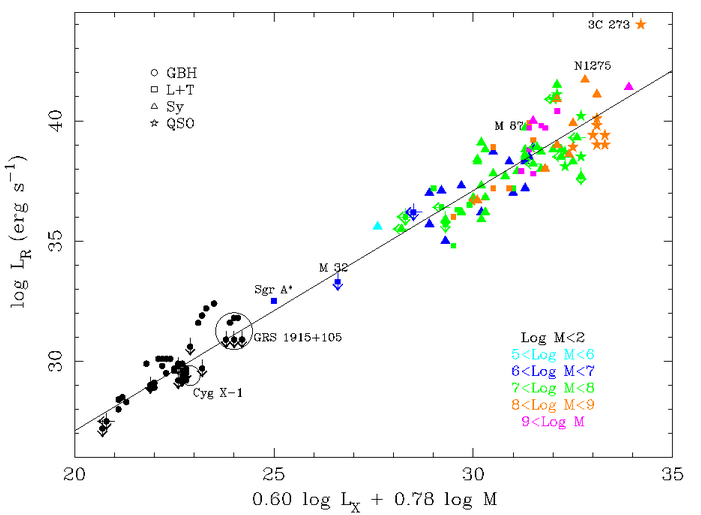
\includegraphics[clip,scale=0.35]{Figures/FP} \protect\caption{\label{fig:Fp}Edge-on view of the fundamental plane from M03 relating
the black hole mass to the radio and X-ray luminosities. Symbols indicate
the type of emission-line galaxy of the host and colors correspond
to the mass of the black hole in units of $\log\left({\rm M}_{\odot}\right)$.
Several well-known galaxies hosting an AGN are listed, as well.}
\end{figure}


The fundamental plane of the BHs relates the mass, X-ray luminosity
and accretion rate. Because the luminosity is not an intrinsic property
of the simulation, it had to be calculated. The calculation of the
luminosity for BH can be approximated by two different models. The
first one takes into account the Eddington luminosity of the BH, which
relates it to the mass, and the second uses the thin disk approximation,
which relates the luminosity to the accretion rate. Both of these
approximations for the luminosity gives the bolometric luminosity.
To get the X-ray luminosity from the bolometric luminosity we use
the \citet{elvis1994atlasof} data sample to calculate a template
. The equation relation from the Elvis template is given by

\begin{equation}
L_{x}=0.1947L_{bol}+1.656\times10^{-15}\;.
\end{equation}


Assuming the BH is only emitting at 10\% off the Eddington luminosity
and by means of the Elvis Template the X-luminosity for the BH is
given by

\begin{equation}
L_{x}=623.04M+1.656\times10^{-15}\;.\label{eq:Lx_propto_m}
\end{equation}
By assuming a thin disk approximation with 10\% efficiency we get
that the X-luminosity for the BH is given by

\begin{equation}
L_{x}=4.64\times10^{19}\dot{M}+1.656\times10^{-15}\;,\label{eq:Lx_propto_mdot}
\end{equation}
for all the cases the masses, accretion rates and luminosities are
measured in $M_{\odot}$, $M_{\odot}s^{-1}$ and $L_{\odot}$. With
equations \ref{eq:Lx_propto_m} and \ref{eq:Lx_propto_mdot} and using
the equation \ref{eq:LxFP}. The fundamental plane equation can be
rewritten in terms of mass, accretion rate, k and q. By means of using
the intrinsic mass to accretion relation, equation \ref{eq:int_relation},
the fundamental plane can be express with only 3 variables.

\begin{multline}
\log\left(9.03\times10^{18}\dot{M}+1.656\times10^{-15}\right)+1.115\log\dot{M}\\
-\frac{e}{d}q\log\dot{M}+k=0
\end{multline}
\begin{multline}
\log\left(623.04+\frac{1.656\times10^{-15}}{M}\right)\\
-0.869q\log M+17.855-k=0
\end{multline}


The parameter $q$ holds the information on the properties of the
BH. Hence the adequate value that fits the simulations had to be found.
Using the Newton-Raphson numerical root-finding method for the two
equations and evaluating throw the whole data sample, $q$ is express
in terms of $k$. We find a high correlation between the values of
$q$ and $k$. Since we hope to reproduce the slope $q$ from M03,
which does not provide typical values for $k$, we must approach this
in a rather roundabout manner. We assume that both approximations
for $L_{x}$ are equally good, and will yield similar results, and
combine \ref{eq:Lx_propto_m} and \ref{eq:Lx_propto_mdot} with the
relationship found between $M$ and $\dot{M}$ given by

\begin{multline*}
\log\left(a_{1}+\frac{b}{M}\right)-dq\log M+eq\\
-\log\left(a_{2}\dot{M}+b\right)+\frac{1}{d}\log\dot{M}-\frac{e}{d}q\log\dot{M}=0\;,
\end{multline*}
where $a_{1}$, $a_{2}$, and $b$ are obtained from converting simulation
units to physical units; and $d$ and $e$ are the slope and the intercept
of the power-law found above. We find that $a_{1}=623.04$, $a_{2}=9.03\times10^{18}$,
$b=1.656\times10^{-15}$, $d=0.869$, and $e=-17.855$.\textbf{These
need units.}

A value of $q$ is found for each black hole by inputting values of
$M$ and $\dot{M}$, and solving for $q$ using Newton-Raphson numerical
root-finding. For the distribution of black holes in our Illustris-2
sample, the distribution of $q$ values is shown in \ref{fig:q_nr_hist}.
The distribution of $q$ values obtained is strongly peaked at around
$.068$, with a mean of $.0693$.

\textbf{What does Figure \ref{fig:Elvis_template} tell us? It's never
mentioned.}
\begin{figure}
\centering{}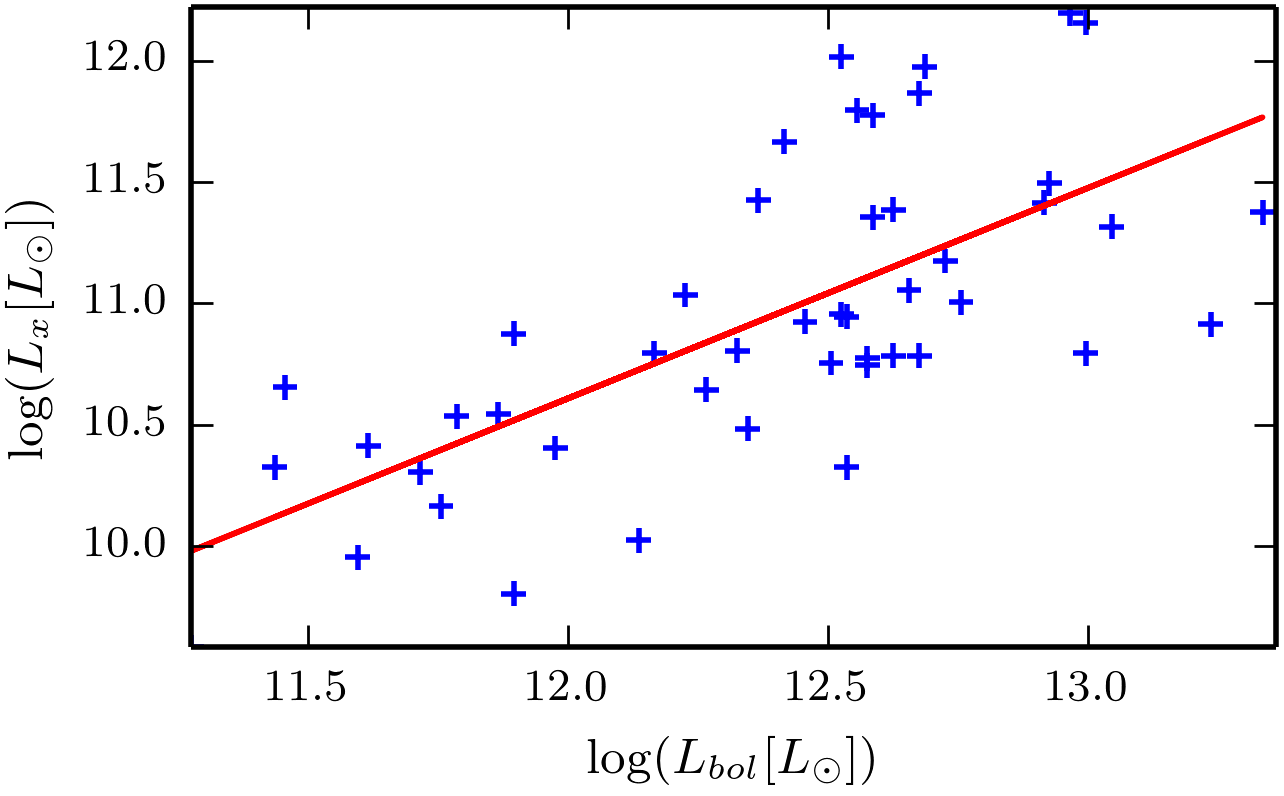
\includegraphics[clip]{Figures/elvis_template} \protect\caption{\label{fig:Elvis_template}The data points from the BH luminosities
over plot with the best-fit linear relation between $L_{x}$ and $L_{bol}$
for the sample.}
\end{figure}
\begin{figure}
\begin{centering}
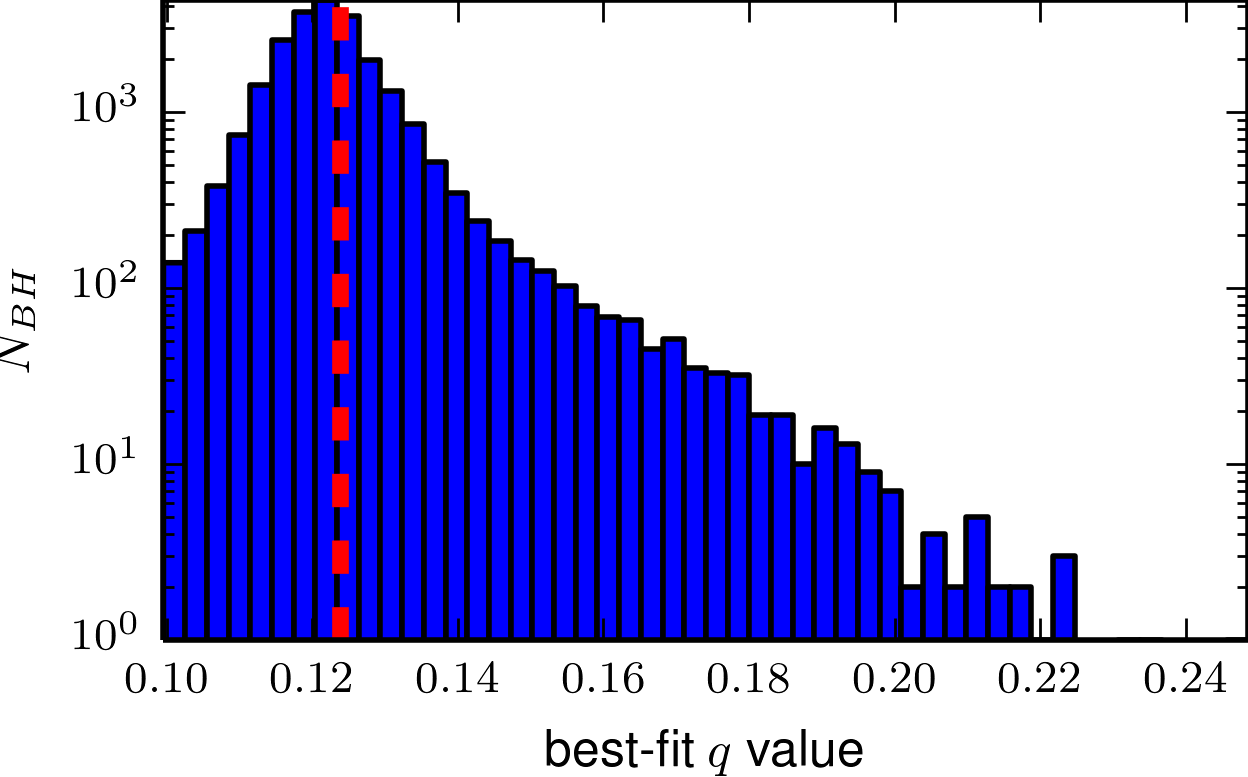
\includegraphics{Figures/q_nr_hist}
\par\end{centering}

\protect\caption{\label{fig:q_nr_hist}A log-histogram of the number of best-fit $q$
values, with one value found per Illustris-2 black hole, using Newton-Raphson
root finding. The maximum likelihood is (SOMEWHERE), with (SOME NUMBER
OF) black holes, and the mean value is $0.693$.}
\end{figure}
